\documentclass{beamer}
\mode<presentation> {
  \usetheme{Darmstadt}
}

\usepackage{graphicx} 
\usepackage{booktabs}
\usepackage{tikz}
\usepackage{amsmath}
\usetikzlibrary{tikzmark}
% Add necessary packages
\usepackage{graphicx}

% set captions with numbers
\setbeamertemplate{caption}[numbered]


\title[2023-2024]{Simple Modeling of Road Traffic.} 

\author{Gerbaud Florent \\ Fatima Rharrour \\ MAM4} 
\institute[Polytech Nice-Sophia] % Your institution as it will appear on the bottom of every slide, may be shorthand to save space
{
Supervisor: \\ % Your institution for the title page
\medskip
{Didier Auroux} % Your email address
}
\date{\today} % Date, can be changed to a custom date
\titlegraphic{
\includegraphics[width=3cm]{Polytech.png}} %
%-----------------------------------------------------------------------------------------
\AtBeginSection[]
{
	\begin{frame}
		\frametitle{Table of Contents}
		\tableofcontents[currentsection]
	\end{frame}
}
\begin{document}

\begin{frame}
\titlepage 
\end{frame}

\begin{frame}
\frametitle{Table of contents} 
\tableofcontents
\end{frame}

%----------------------------------------------------------------------------------------
%	PRESENTATION SLIDES
%----------------------------------------------------------------------------------------

%------------------------------------------------
\section{Introduction:} 
%------------------------------------------------
\begin{frame}
        \subsection{Presentation of the subject}
	\frametitle{Presentation of the subject:}
        \begin{center}
        \textbf{What is Road Traffic Modelling?}
         \end{center}
	
        
	\begin{columns}
		\column{0.6\textwidth}
		\begin{itemize}
			\item Representing complex dynamics of vehicles moving along roads.
			\item Creating mathematical and computer models for:
			\begin{itemize}
				\item Understanding vehicle flow.
				\item Predicting movement patterns.
				\item Analyzing interactions on roads and highways.
			\end{itemize}
		\end{itemize}
		
		\column{0.4\textwidth}
		\begin{center}
			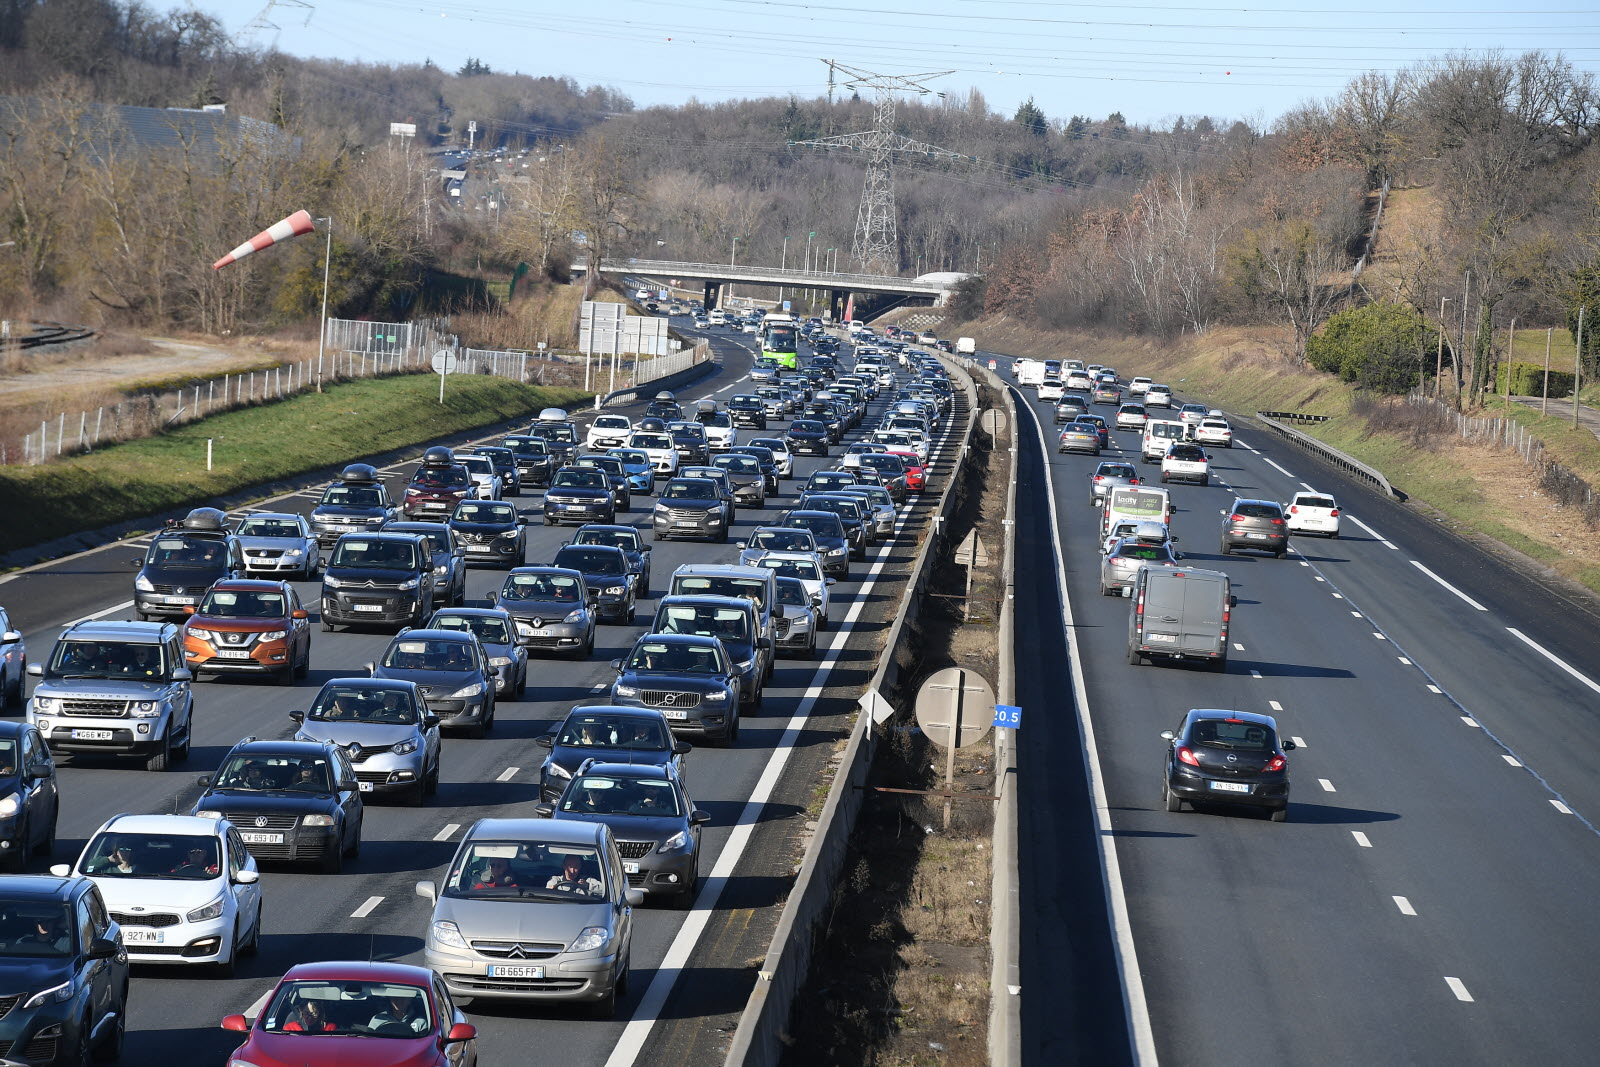
\includegraphics[width=\textwidth]{PIC1.jpg}
			\tiny{\textit{Fig. 1: Real-life Road Traffic}}
		\end{center}
	\end{columns}
\end{frame}

%******************************************************************************************
\begin{frame}
        \frametitle{Presentation of the subject:}
	\begin{block}{Key benefits of Road Traffic Modeling:}
		\begin{itemize}
	\item \textbf{Avoiding traffic jams:} Helps find solutions to prevent traffic jams on roads.
	\item \textbf{Making Roads Better:} Finds ways to improve roads and make them work smoother.
	\item \textbf{Understanding how traffic works:} Helps figure out how different things affect traffic and predict what might happen.
	\item \textbf{Making transportation better:} Shows how well transportation works and helps make it even better.
	\item \textbf{Saving time and money:} Aims to reduce time spent waiting in traffic and the money spent on each trip.
\end{itemize}
	\end{block}
\end{frame}
%******************************************************************************************
\begin{frame}{Presentation of the subject}
    Animation à ajouter ??
\end{frame}
%******************************************************************************************
\begin{frame}
\subsection{Project organization overview}
\frametitle{Project organization overview}
\begin{center}
    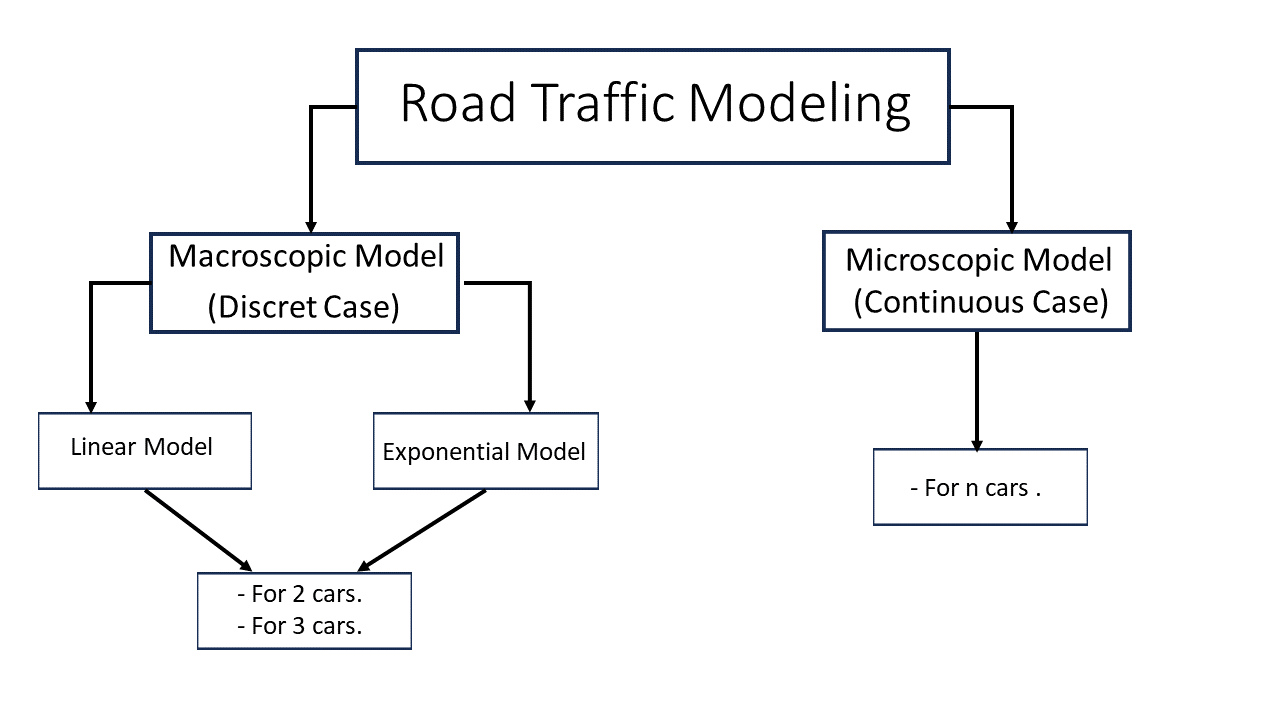
\includegraphics[width=1\textwidth]{org1.png} 
    \end{center}
\end{frame}
%******************************************************************************************

\begin{frame}{Useful definitions:}
        \subsection{Useful definitions}
	\vspace{-0.2cm}
	\begin{block}{Microscopic simulation:}
		Microscopic simulation is a computer-based modeling technique that simulates the behavior of individual entities, such as vehicles or pedestrians, within a system
	\end{block}
	\vspace{-0.2cm}
	\begin{block}{Macroscopic simulation:}
		Macroscopic simulation models systems at a higher, aggregated level, considering overall behaviors like traffic flow without detailing individual movements.
	\end{block}
	\vspace{-0.2cm}
	\begin{block}{Ordinary Differential Equation (ODE) :}
		An ODE is a mathematical equation that relates a function to its derivatives with respect to one or more independent variables.
		\[
		F\left(x,y,y',\ldots ,y^{(n-1)}\right)=y^{(n)}
		\]
	\end{block}
\end{frame}

%------------------------------------------------
\section{Study of the discret case:}
%------------------------------------------------

\begin{frame}{Ordinary Differential Equation (Theory):}
\subsection{Ordinary Differential Equation}
\begin{figure}
    \centering
    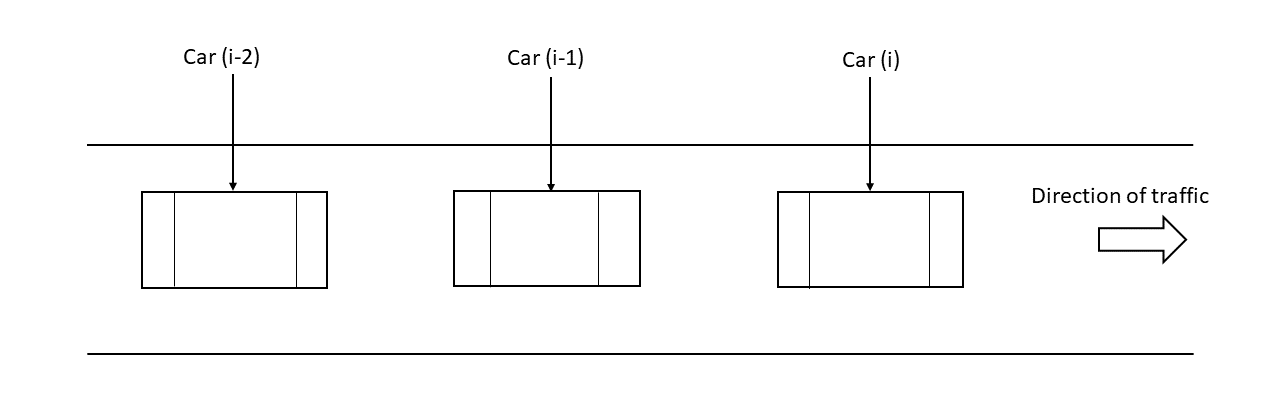
\includegraphics[width=0.6\textwidth]{discret.png} 
    \caption{ Discret Model.}
\end{figure}
\vspace{-0.7cm}
\begin{block}{ODE to solve}
	\begin{center}
		$\boxed{\mathbf{y'(t) = f{\bigl (}t, y(t){\bigr )}}}$
	\end{center}
	Euler Explicit method to numerically solve the solutions:
	\begin{itemize}
		\item First step of the resolution: $\boxed{y_0 = y(t_0)}$.
		\item Recursive process to find the n-th solution of the ODE: $\boxed{y_{n+1} = y_{n} + hf(t_{n}, y_{n})}$
	\end{itemize}
\end{block}


    
\end{frame}
\begin{frame}
\subsection{Velocity modeling: The linear approach}
\frametitle{Velocity modeling: The linear approach}

    \begin{alertblock}{Each car's movement is governed by the basic equation}
    	\[
    	\boxed{\dot{x_i}(t) = V_i = \alpha_i(x_{i-1} - x_i)}
    	\]
    \end{alertblock}
    
    \begin{block}{Where}
    	\begin{center}
    		\begin{tabular}{l l}
    			\(\dot{x_i}(t)\): & Instantaneous velocity of the \(i\)-th car at time \(t\) \\
    			\(V_i\): & Current velocity of the \(i\)-th car \\
    			\(\alpha_i\): & Coefficient describing the behavior of the \(i\)-th car \\
    			\(x_{i-1}\): & Previous position of the \(i\)-th car \\
    			\(x_i\): & Current position of the \(i\)-th car
    		\end{tabular}
    	\end{center}
    \end{block}
\end{frame}

\begin{frame}{Velocity Modeling: The Linear Approach}
	\begin{block}{System of Equations for $N$ cars}
		\[
		\left\{
		\begin{array}{ll}
			\dot{x}_1 &= V_1 \\
			\dot{x}_2(t) &= \alpha_2(x_1 - x_2) \\
			&\vdots \\
			\dot{x}_n(t) &= \alpha_n(x_{n-1} - x_n)
		\end{array}
		\right.
		\]
	\end{block}
	
	\begin{block}{Systems for Positions of N cars}
		\begin{align*}
			\left\{
			\begin{array}{ll}
				x_1(t + \Delta t) &= x_1(t) + \Delta t  \cdot V_1\\
				x_2(t + \Delta t) &= x_2(t) + \Delta t  \cdot \alpha_2(x_1 - x_2) \\
				&\vdots \\
				x_n(t + \Delta t) &= x_n(t) + \Delta t \cdot  \alpha_n(x_{n-1} - x_n)
			\end{array}
			\right.
		\end{align*}
	\end{block}
	
\end{frame}

\begin{frame}{Velocity Modeling: The Newell Approach}
\subsection{Velocity Modeling: The Newell Approach}

\begin{alertblock}{Each car's movement is described by the equation}
	\[
	\boxed{\dot{x_i}(t) = V_i\left( 1 - e^{-\frac{\lambda_i}{V_i}(x_{i-1}(t) - x_i(t) - d_i)}\right) }
	\]
\end{alertblock}

\begin{block}{Where}
	\begin{center}
		\begin{tabular}{l l}
			\(V_i\): & the maximum velocity of the \(i\)th car \\
			\(\lambda_i\): & the capacity of acceleration/deceleration \\
			\(d_i\): & safe following distance associated with the \(i\)th car \\
		\end{tabular}
	\end{center}
\end{block}

\end{frame}
\begin{frame}{Velocity Modeling: The Newell Approach}
		\vspace{-0.3cm}
    	\begin{block}{System of Equations for $N$ cars}
    	\begin{align*}
    		\left\{
    		\begin{array}{ll}
    			\dot{x}_1 &= V_1 \\
    			\dot{x}_2(t) &= V_2(1-e^{-\frac{\lambda_2}{V_2}(x_{1}(t) - x_2(t) - d_2}) \\
    			&\vdots \\
    			\dot{x}_n(t) &= V_n(1-e^{-\frac{\lambda_n}{V_n}(x_{n-1}(t) - x_n(t) - d_n})
    		\end{array}
    		\right.
    	\end{align*}
    \end{block}
    \vspace{-0.3cm}
    \begin{block}{Systems for Positions of N cars}
    	\begin{align*}
    		\left\{
    		\begin{array}{ll}
    			x_1(t + \Delta t) &= x_1(t) + \Delta t \cdot  V_1\\
    			x_2(t + \Delta t) &= x_2(t) + \Delta t \cdot V_2(1-e^{-\frac{\lambda_2}{V_2}(x_{1}(t) - x_2(t) - d_2}) \\
    			&\vdots \\
    			x_n(t + \Delta t) &= x_n(t) + \Delta t \cdot V_n(1-e^{-\frac{\lambda_n}{V_n}(x_{n-1}(t) - x_n(t) - d_n})
    		\end{array}
    		\right.
    	\end{align*}
    \end{block}
\end{frame}
\begin{frame}{Accordion phenomenon}
	\subsection{Simulations}
	\begin{minipage}{0.48\textwidth}
		\centering
		\begin{figure}
			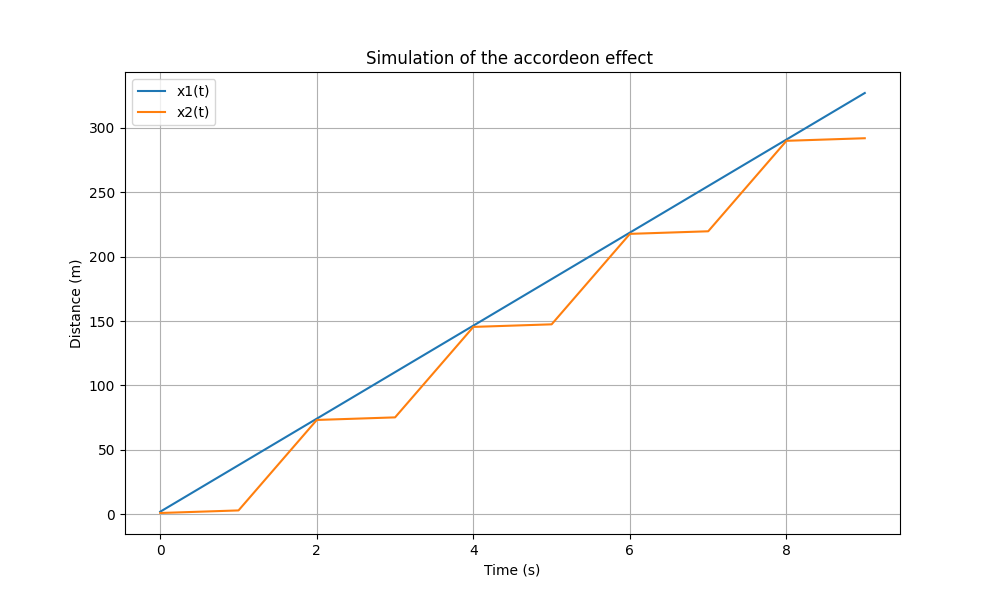
\includegraphics[width=\textwidth]{Accordeon1.png}
			\caption{Modelisation of the accordion phenomenon with The Linear Model}
			\label{fig:AL}
		\end{figure}
	\end{minipage}\hfill
	\begin{minipage}{0.48\textwidth}
		\centering
		\begin{figure}
			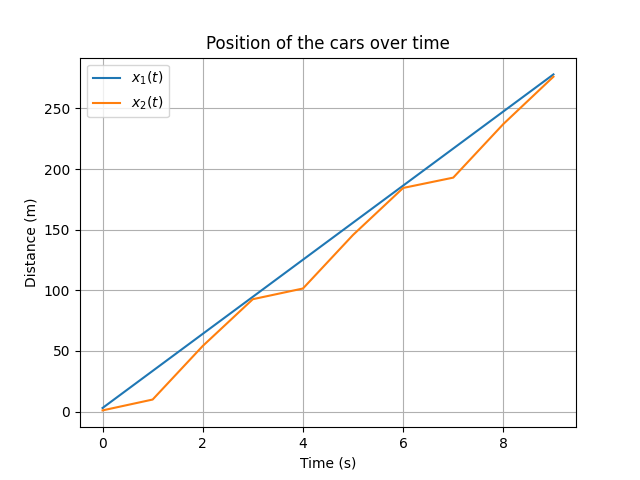
\includegraphics[width=\textwidth]{1W2_Accord.png}
			\caption{Modelisation of the accordion phenomenon with The Newell's Model}
			\label{fig:AN}
		\end{figure}
	\end{minipage}
	\begin{block}{}
		We could see the difference of modelisation and realism between the Linear model (figure \ref{fig:AL}) and the Newell's model (figure \ref{fig:AN})
	\end{block}
\end{frame}
\begin{frame}{Drunk drivers }
	\begin{minipage}{0.49\textwidth}
		\centering
		\begin{figure}
			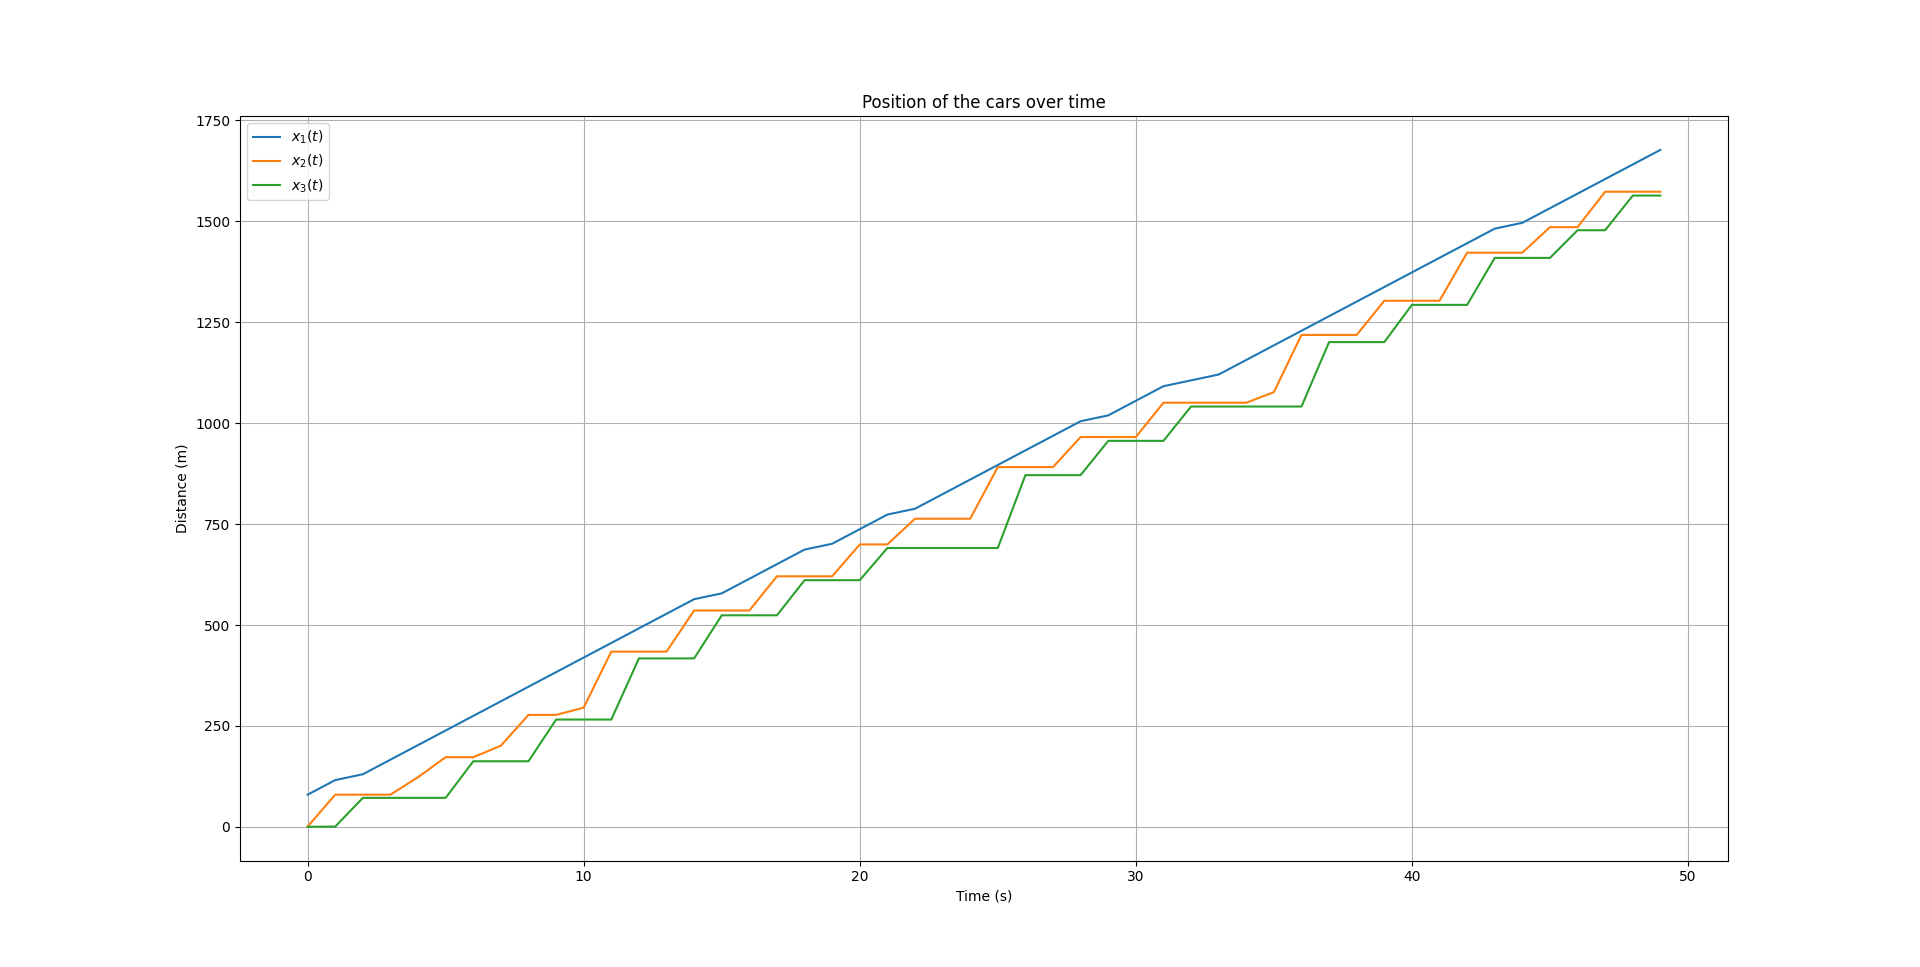
\includegraphics[width=1.1\textwidth]{Model1W3C_O_Aco_D2_Linear.png}
			\caption{Simulation of Traffic Flow with one drunk driver (Linear Model)}
			\label{fig:DL}
		\end{figure}
	\end{minipage}\hfill
	\begin{minipage}{0.49\textwidth}
		\centering
		\begin{figure}
			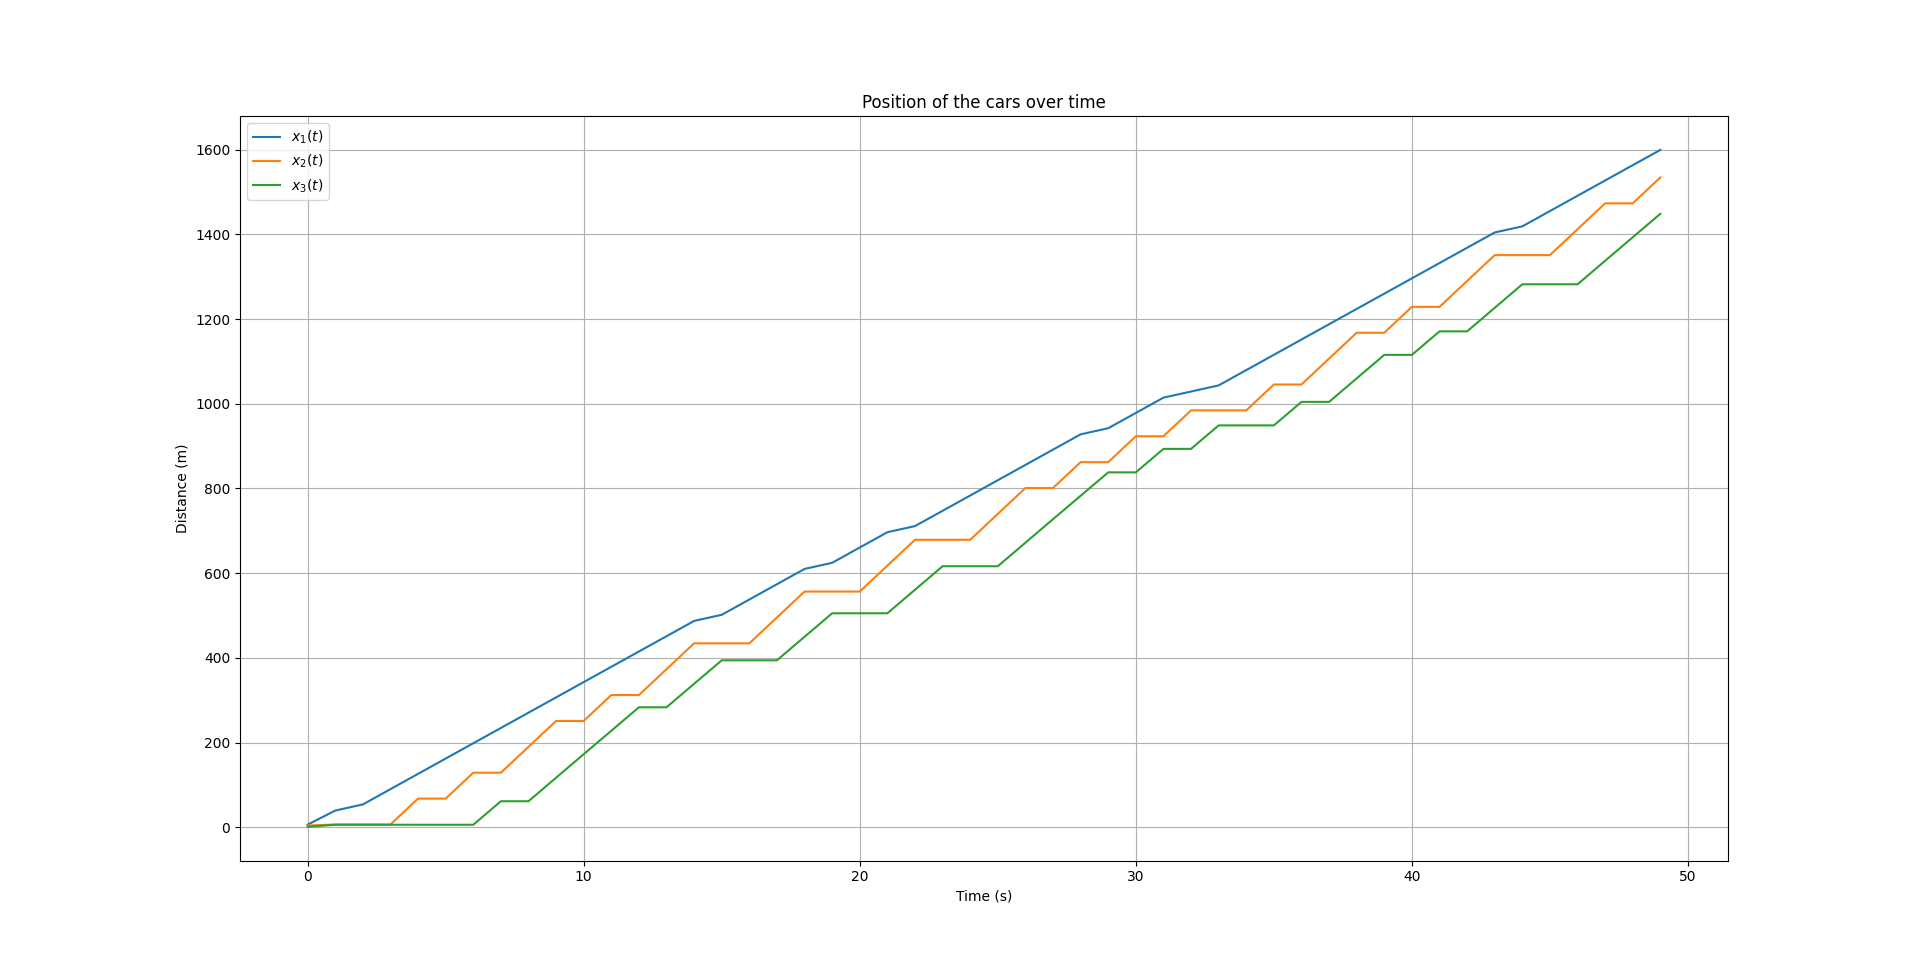
\includegraphics[width=1.1\textwidth]{Model1W3C_O_Aco_D2_Newell.png}
			\caption{Simulation of Traffic Flow with one drunk driver (Newell's Model)}
			\label{fig:DN}
		\end{figure}
	\end{minipage}
	\begin{block}{}
		It is interesting to note that with Newell's Method (Figure \ref{fig:DN}), the variations are "smoothed and much less significant than in the case of the linear method (\ref{fig:DL})."
	\end{block}
\end{frame}

\begin{frame}{Accident phenomenon}
    \begin{figure}
    	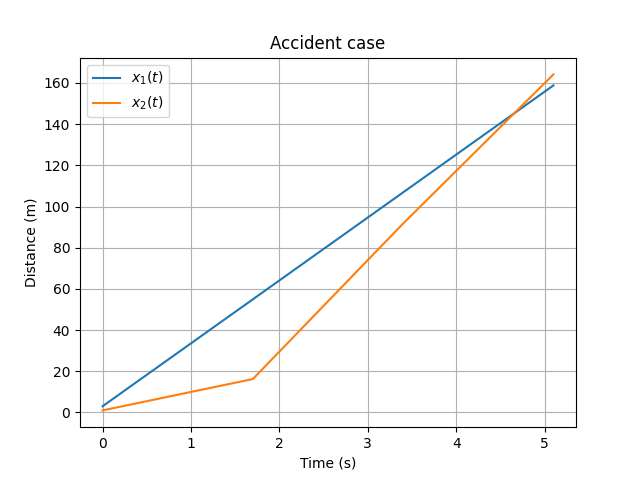
\includegraphics[width=0.5\textwidth]{1W2_Acc2.png}
    	\caption{Modelisation of the accordion phenomenon with The Newell's Model}
    	\label{fig:ACC}
    \end{figure}
    \begin{block}{}
    	On the figure \ref{fig:ACC}, you can see that when the curves intersect, there is an accident
    \end{block}
\end{frame}
%Cas des 3 voitures !!
\subsection{Study of Equilibrium and Stability}
\subsubsection{Using linear model:}
\begin{frame}{Analytical Solutions}
	\begin{figure}[H]
		\centering
		\begin{minipage}[t]{0.49\linewidth}
			\centering
			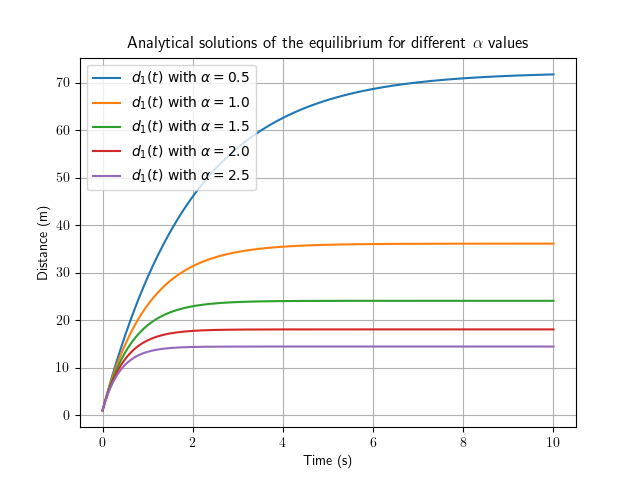
\includegraphics[width=\linewidth]{Stability.png}
			\caption{Stability Analysis for Three Cars}
			\label{fig:StabilityAnalysis}
		\end{minipage}
		\begin{minipage}[t]{0.49\linewidth}
			\centering
			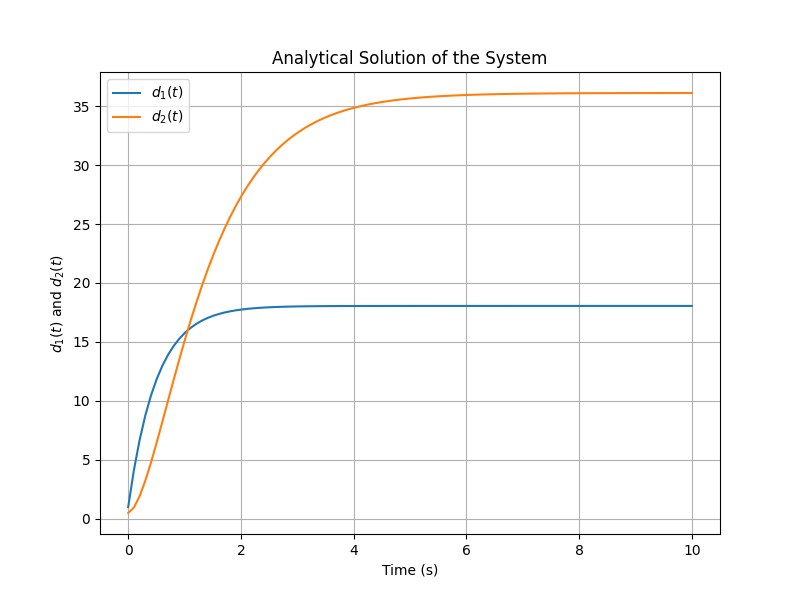
\includegraphics[width=\linewidth]{AnalyticalSolution.png}
			\caption{Analytical Solution for Three Cars}
			\label{fig:AnalyticalSolution}
		\end{minipage}\hfill
		\label{fig:CombinedFigures}
	\end{figure}
\end{frame}

\begin{frame}{Equilibrium}
	\begin{figure}[H]
		\centering
		\begin{minipage}[t]{0.46\textwidth}
			\centering
			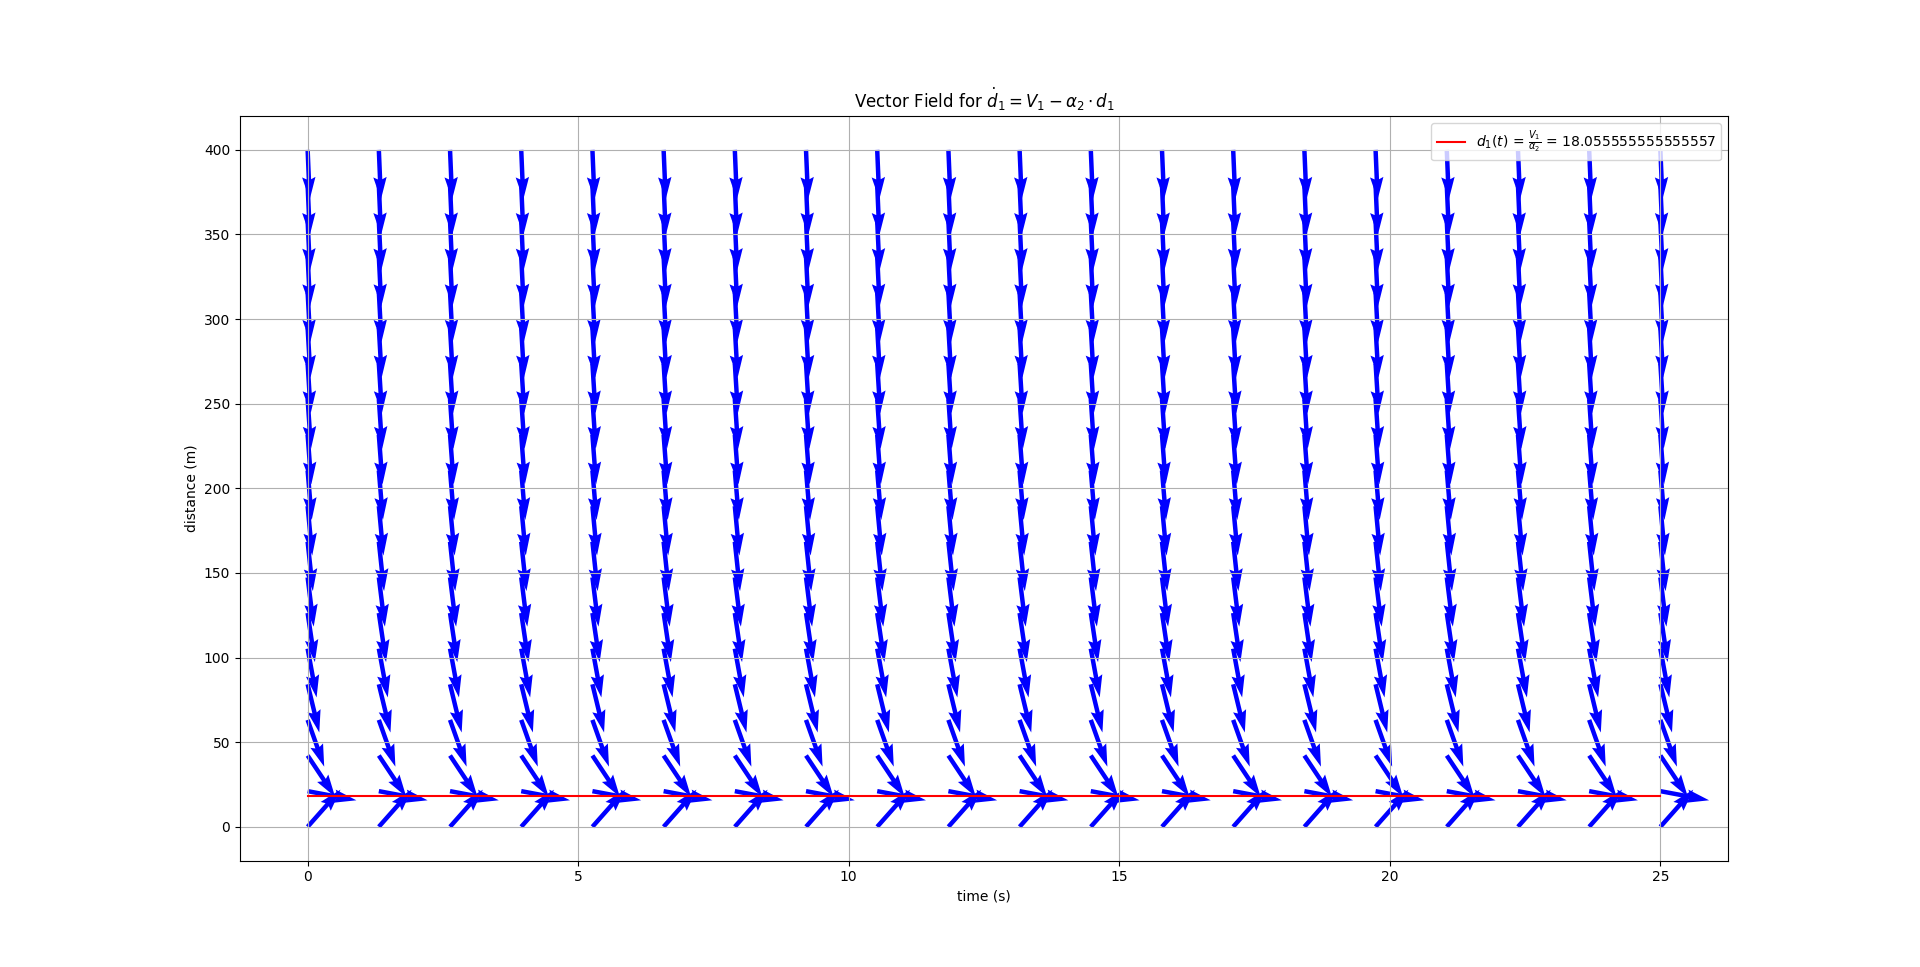
\includegraphics[width=1\linewidth]{FieldOfVector_CV.png}
			\caption{Field Of Vector for the Newell's Model (Stability)}
		\end{minipage}
		\hfill 
		\begin{minipage}[t]{0.51\textwidth}
			\centering
			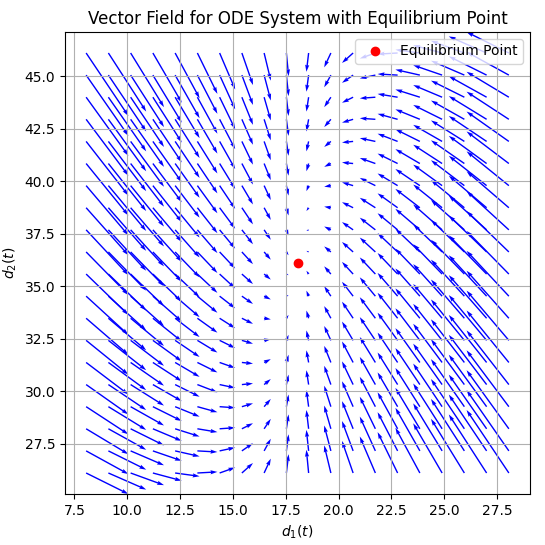
\includegraphics[width=0.9\linewidth]{FieldOfVector_CV2.png}
			\caption{Field Of Vector for the Linear Model (Stability)}
			\label{fig:FV1}
		\end{minipage}
		\label{fig:CombinedFigures}
	\end{figure}
\end{frame}



\subsubsection{Using the Newell's model}
\section{Study of the continuous model:}
\begin{frame}{Mathematical Theory}
	\begin{alertblock}{Conservation Law}
		\begin{itemize}
			\item $\partial_t\rho + \partial_x\left[ \rho\left( 1-\frac{\rho}{\rho_{\text{max}}}\right) \cdot V_{\text{max}}\right] = 0 $
		\end{itemize}
	\end{alertblock}
	\begin{block}{Initial and Boundary Conditions}
		\begin{itemize}
			\item $\rho(x,0) = \rho_0(x), \quad x \in \Omega,$
			\item $\rho(0,t) = \rho(L,t), \quad t \geq 0$
			\item $\Omega := \left] 0,L\right[, $
			\item $\rho(x,t)$ represents the traffic density at position $x$ and time $t$, 
			\item $F(\rho)$ denotes the traffic flux as a function of density,
			\item $F(\rho)$ is often represented by a function modeling the relationship between traffic density and traffic velocity,
			\item $F(\rho) = V(\rho) \cdot \rho,$ where $V(\rho)$ is the traffic velocity as a function of density.
		\end{itemize}
	\end{block}
\end{frame}

\subsection{Euler Explicit Method}
\begin{frame}{Numerical Scheme for the resolution}
	\begin{alertblock}{Numerical Scheme}
		\begin{itemize}
			\item $\rho_{i}^{n+1} = \rho_i^n - \frac{\Delta t}{\Delta x} \cdot \left(\rho_i^n \cdot v_i^n - \rho_{i-1}^n \cdot v_{i-1}^n \right)
					=0$
		
			\item $v_i^n = \left( 1 - \frac{\rho_i^n}{\rho_{max}}\right)  \times V_{max}$
		\end{itemize}
	\end{alertblock}
	enrichir la slide. Peut etre ajouter le modèle dans la théorie et dire que quand on l'applique on obtient ca ou alors mettre une iage qui explique le shéma de Euler explicit ? 

	%slide : 
%Partie Math EDP
%Equation + cond au bord
%petite def de ce qu’il y a dans l’équation
\end{frame}

\begin{frame}
	\begin{figure}[H]
		\centering
		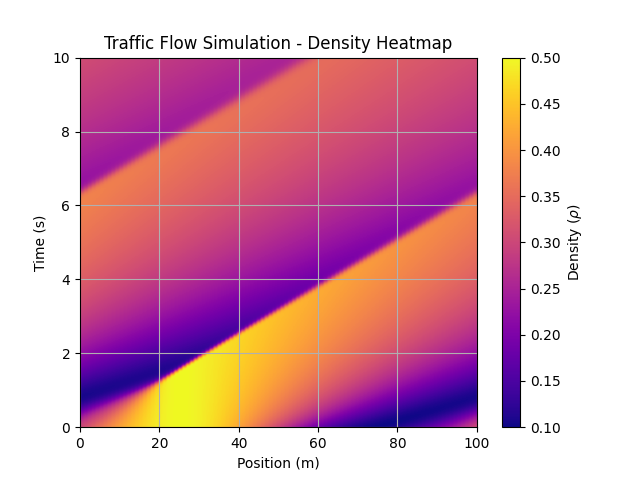
\includegraphics[width=0.65\textwidth]{traffic_flow_density_map.png}
		\caption[Traffic Flow Simulation With Euler Explicit]{\textbf{\underline{Traffic Flow Simulation With Euler Explicit:}} This figure illustrates the solution of the PDE at any time and position. Here is the link to the associated animation showing the movement of the traffic flow: \href{https://github.com/FlorentGerbaud/Simple-road-traffic-modeling/blob/Flo-PDE/SRTM/EDPMethod/CasTestToLaunch/TestToLaunch/Modele_IC_S/EulerExplicit/traffic_flow_animation.gif}{\textbf{\underline{Traffic Flow Simulation}}} }
		\label{fig:traffic_flow_density_map}
	\end{figure}
\end{frame}

\subsection{Lax-Friedrichs method}
\begin{frame}{Numerical Scheme for the resolution}
	\begin{alertblock}{Numerical Scheme}
		\begin{equation*}
			\begin{split}
				\rho_{j}^t &= \frac{1}{2} \left(\rho_{j+1}^{t-1} + \rho_{j-1}^{t-1}\right) 
			 - \frac{\Delta t}{2 \cdot \Delta x} \left( \rho_{j+1}^{t-1} \left(1 - \frac{\rho_{j+1}^{t-1}}{\rho_{max}}\right) \cdot V_{\text{max}} \right. \\
				&\quad \left. - \rho_{j-1}^{t-1} \left(1 - \frac{\rho_{j-1}^{t-1}}{\rho_{max}}\right) \cdot V_{\text{max}} \right)
			\end{split}
		\end{equation*}
		
	\end{alertblock}
	enrichir la slide. Peut-être ajouter le modèle dans la théorie et dire que quand on l'applique on obtient ça ou alors mettre une image qui explique le schéma de Euler explicite ? 
	
	%slide: 
	%Partie Math EDP
	%Equation + cond au bord
	%petite définition de ce qu’il y a dans l’équation
\end{frame}


\begin{frame}
	\begin{figure}[H]
		\centering
		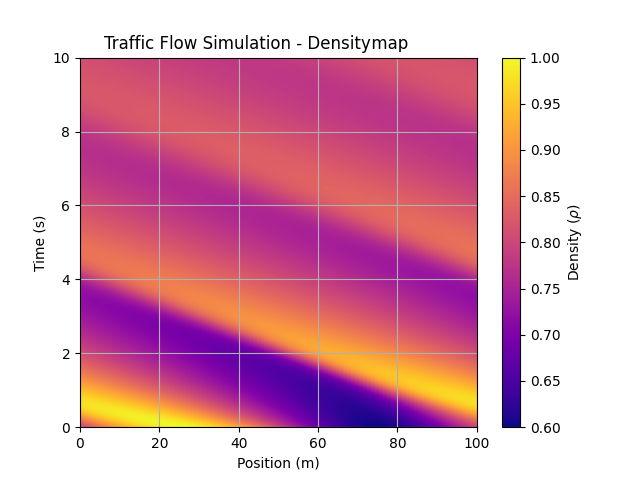
\includegraphics[width=0.65\textwidth]{traffic_flow_density_map_LF.png}
		\caption[Traffic Flow Simulation With Euler Explicit]{\textbf{\underline{Traffic Flow Simulation With Euler Explicit:}} This figure illustrates the solution of the PDE at any time and position. Here is the link to the associated animation showing the movement of the traffic flow: \href{https://github.com/FlorentGerbaud/Simple-road-traffic-modeling/blob/Flo-PDE/SRTM/EDPMethod/CasTestToLaunch/TestToLaunch/Modele_IC_S/LaxFriedrichs/traffic_flow_animation.gif}{\textbf{\underline{Traffic Flow Simulation}}} }
		\label{fig:traffic_flow_density_map}
	\end{figure}
\end{frame}

\section{Conclusion}

\end{document}